\documentclass[10pt,a4paper]{article}
\usepackage[UTF8]{ctex}
\usepackage{amsmath,amssymb}
\usepackage{graphicx}
\usepackage{booktabs}
\usepackage{array}
\usepackage{geometry}
\usepackage{caption}
\usepackage{subcaption}
\usepackage{enumitem}
\usepackage{float}
\usepackage{xcolor}
\usepackage{hyperref}
\usepackage{listings}
\usepackage{anyfontsize}

\geometry{margin=1.8cm}
\hypersetup{colorlinks=true,linkcolor=black,citecolor=black,urlcolor=blue}
\captionsetup{font=small,labelfont=bf}
\setlist[itemize]{nosep,leftmargin=1.5em}
\setlength{\tabcolsep}{4pt}
\renewcommand{\arraystretch}{1.12}
\linespread{1.0}
\setlength{\emergencystretch}{3em}
\newcommand{\figgpu}[1]{\includegraphics[width=0.8\linewidth]{../files/figures/gpu_report/#1.pdf}}
\newcommand{\msq}{ms/query}
\lstset{
    basicstyle=\ttfamily\footnotesize,
    breaklines=true,
    frame=single,
    showstringspaces=false,
    columns=fullflexible,
    keepspaces=true
}
\emergencystretch=2em

\begin{document}
\fontsize{9.2pt}{10.9pt}\selectfont

\title{\textbf{HIP 基础学习与 GPU ANN 批查询加速}\\
\large HIP 编程模型、矩阵乘法、IVF 批处理与精度--延迟权衡}
\author{}
\date{}
\maketitle
\thispagestyle{empty}
\vspace{-1.8em}
\begin{center}
{\renewcommand{\arraystretch}{1.25}
\begin{tabular*}{0.82\textwidth}{@{\extracolsep{\fill}}>{\bfseries}l l >{\bfseries}l l@{}}
姓名 & 匡航逸 & 学号 & 2412235 \\
专业 & 计算机科学与技术 & 日期 & \today \\
GitHub & \multicolumn{3}{l}{\href{https://github.com/xzxxntxdy/Parallel-programming-NKU}{https://github.com/xzxxntxdy/Parallel-programming-NKU}} \\
\end{tabular*}}
\end{center}
\vspace{0.2em}

\begin{abstract}
\small
本文首先整理 AMD AUP HIP 基础课程中 Vector Addition、Matrix Transpose、Histogram、Reduction、Monte Carlo Integration 与 K-Means Clustering 六个实验的代码填空和分析答案，覆盖 HIP 线程索引、wavefront 对齐、shared memory、atomic、grid-stride loop、归约和迭代算法等核心概念。进阶部分针对 DEEP100K 内积 ANN 查询实现并评测 GPU 批处理加速方案。GPU 很难有效加速单个查询，因此实现以 query batch 为基本单位：一条路线将 exact flat scan 表示为 $N\times d$ base 矩阵与 $d\times m$ query 矩阵的乘法，并比较 naive CUDA kernel、shared-memory tiling kernel 与 cuBLAS SGEMM；另一条路线实现 IVF，先用 coarse centroid 将 base 划分为倒排簇，再对每个 query 的 $nprobe$ 个簇进行 GPU 距离计算。为分析 IVF 批处理中不同 query 探测簇不一致造成的浪费，本文同时实现了按簇矩阵批处理 baseline、按最近中心排序的 query grouping，以及候选列表压缩的 compact kernel。所有正式实验在本地 NVIDIA GeForce RTX 4060 Laptop GPU 上完成，指标固定为 recall@100 与单 query latency。最终在 recall@100$\ge0.95$ 的约束下，CUDA IVF compact 以 $nlist=256,nprobe=20,batch=32$ 达到 0.1201~\msq{}、recall@100=0.9510；相比 CPU exact scan 的 3.3154~\msq{} 提升 27.6$\times$，相比 cuBLAS exact scan 的 0.1778~\msq{} 提升 1.48$\times$。实验表明，GPU ANN 的主要收益来自批量距离计算与候选数下降，而最终延迟受 top-k、host--device 传输、batch padding 和簇级 kernel launch 共同限制。
\end{abstract}


\section{HIP 基础学习内容}

HIP 基础部分围绕 AMD AUP 的六个实验展开，覆盖 Vector Addition、Matrix Transpose、Histogram、Reduction、Monte Carlo Integration 与 K-Means Clustering。本节按实验顺序概括各章涉及的并行编程知识；具体填空、计算题和问答题见附录~\ref{app:hip-answers}。表~\ref{tab:hip-learning-map} 先概括各章节的学习主题，后续小节再展开说明。

\begin{table}[H]
\centering
\small
\caption{HIP 六个基础实验的学习主题与附录对应位置。}
\label{tab:hip-learning-map}
\begin{tabular}{p{0.22\linewidth}p{0.44\linewidth}p{0.22\linewidth}}
\toprule
章节 & 主要学习内容 & 题目与答案位置 \\
\midrule
Vector Addition & 线程层次、全局索引、边界检查、launch configuration、wavefront 与 occupancy & 附录~\ref{app:hip-answers}，A.1 \\
Matrix Transpose & 二维索引、row-major 地址映射、coalesced access、shared-memory tile 与 bank conflict & 附录~\ref{app:hip-answers}，A.2 \\
Histogram & naive 并行统计的重复读、shared-memory 局部直方图、atomic contention 与输入分布影响 & 附录~\ref{app:hip-answers}，A.3 \\
Reduction & tree reduction、同步必要性、occupancy 的局限、final atomic 次数与 block size 权衡 & 附录~\ref{app:hip-answers}，A.4 \\
Monte Carlo Integration & atomic reduction 瓶颈、shared-memory reduction、grid-stride loop、浮点累加精度 & 附录~\ref{app:hip-answers}，A.5 \\
K-Means Clustering & assignment/update 两阶段、shared/global atomic 分层、centroid 缓存、收敛检测与双缓冲 & 附录~\ref{app:hip-answers}，A.6 \\
\bottomrule
\end{tabular}
\end{table}

从学习路径看，这六个实验不是彼此独立的填空题，而是从“单元素并行”逐步过渡到“结构化并行算法”的过程。Vector Addition 只要求线程和数组元素一一对应，重点是索引正确性、边界检查和 launch configuration；Matrix Transpose 开始引入二维数据布局，使同样的线程数量在不同访存方向下产生完全不同的带宽效率；Histogram 和 Reduction 则把多个线程写入同一结果的问题显式暴露出来，要求用 atomic、shared memory 和同步来控制数据竞争；Monte Carlo 与 K-Means 进一步把归约放入数值计算和迭代算法中，强调并行程序不仅要跑得快，还要保持数值稳定和状态一致。

因此，HIP 基础学习的核心不是记住某个 kernel 模板，而是形成一套检查 GPU 程序的顺序。首先确认每个线程负责哪一个数据元素或哪一段数据，避免越界和重复写；其次检查 global memory 访问是否连续、是否合并、是否被重复扫描放大；然后判断是否存在多个线程写同一地址的情况，并选择 shared-memory 局部聚合、global atomic 或分阶段归约；最后再用 occupancy、memory bandwidth、atomic contention 和 kernel launch 开销解释性能。这个顺序贯穿附录~\ref{app:hip-answers} 中的计算题与问答题，也为后续 ANN GPU 实验中的 batch 并行和候选压缩提供了分析框架。

\subsection{Vector Addition：线程层次与最小 kernel}

Vector Addition 是 HIP 学习中的入口实验，核心价值在于把 GPU 的抽象执行模型落到一个最小可验证 kernel 上。通过该实验可以明确 grid、block、thread 三层层次如何映射到数组元素：线程使用 \texttt{blockIdx.x * blockDim.x + threadIdx.x} 计算全局索引，再用 \texttt{idx < N} 做边界保护。这个边界判断并不是附加细节，而是 GPU kernel 正确性的基本组成部分，因为实际 launch 的线程总数通常是 block size 的整数倍，而输入规模并不一定整除 block size。

该实验还引入了 launch configuration 的计算方式。给定 $N=1000$，block size 为 64、128、256、512 时都会产生 1024 个总线程，空闲线程均为 24，线程利用率相同。这一结果说明，单纯从“是否浪费线程”判断 block size 是不充分的；真实性能还受 wavefront 对齐、寄存器使用、LDS 使用、每 CU 可驻留 block 数和调度开销影响。Vector Addition 每个元素只执行一次加法，却需要两个 global memory read 和一个 global memory write，因此它更接近 memory bandwidth bound kernel，而不是 compute bound kernel。这个判断方法比具体某个 block size 的结果更重要。

Vector Addition 的后半部分讨论 wavefront 与 occupancy。RDNA 默认 wave32 时，小于 32 的 block size 会形成 sub-wavefront，部分 lane 空闲但仍占用调度资源；wave64 模式下，对齐目标又会改变。occupancy 章节进一步说明，active wavefront 数达到上限并不自动代表最快，因为隐藏访存延迟只是性能的一部分，指令开销和访存形态同样会影响结果。完整的计算表和具体填空见附录~\ref{app:hip-answers} 的 A.1。

这一章还建立了 host--device 程序的基本生命周期：host 端分配并初始化数据，使用 \texttt{hipMalloc} 在 device 上申请显存，通过 \texttt{hipMemcpy} 完成输入输出传输，随后以 \texttt{hipLaunchKernelGGL} 启动 kernel。由于 kernel launch 是异步的，计时和结果读取前需要用同步或事件保证 GPU 工作已经完成。这个流程看似简单，却是后续所有实验的共同骨架；如果漏掉同步，计时会低估 kernel 时间，如果遗漏边界保护，最后一个不完整 block 会导致非法访问或错误结果。

\subsection{Matrix Transpose：二维索引与访存合并}

Matrix Transpose 将一维数组映射扩展到二维矩阵。实验首先根据 block index、thread index 与 $32\times32$ 的 block 形状计算二维全局坐标 $(idx,idy)$，再把坐标转换成 row-major 地址。这个过程强化了两个基本事实：一是 GPU 线程的维度只是组织方式，最终仍要转换为线性内存地址；二是矩阵转置改变的是输出矩阵的行列关系，输出下标必须使用 $idx\times rows+idy$，而不是 $idx\times cols+idy$。

该实验最关键的学习点是 coalescing。朴素转置读取 \texttt{input[idy * cols + idx]} 时，同一 wavefront 中连续 \texttt{idx} 读取连续地址，global memory transaction 可以合并；但写入 \texttt{output[idx * rows + idy]} 时，连续线程之间的地址 stride 为 $rows$ 个 float。对 $1024\times1024$ 矩阵，这个 stride 是 4096 bytes，一个 wavefront 的 32 个线程会落在不同 128-byte 区域，写入无法合并。由此可以看到，算法上只交换行列很简单，但在 GPU 上读写方向不同会导致完全不同的内存效率。

tiled transpose 用 shared memory 解决这个问题。每个 block 先把一个 tile 从 global memory 连续读入 LDS，再在 shared memory 中完成局部转置，最后按连续地址写回输出矩阵。实验中的片上数组采用
\begin{center}
\small\texttt{tile[BLOCK\_SIZE][BLOCK\_SIZE+1]}
\end{center}
这样的布局，第二维的 $+1$ padding 用于改变 shared memory 行 stride，减少转置访问时的 bank conflict。该章学习到的重点不是“转置”本身，而是如何通过片上存储改变 global memory 的访问顺序。具体索引计算、transaction 数量和 shared memory 用量见附录~\ref{app:hip-answers} 的 A.2。

\subsection{Histogram：并行统计与 atomic contention}

Histogram 章节展示了并行算法设计中“看似并行但实际低效”的典型情形。naive 版本让每个 block 负责一个 bin，并让每个 block 扫描完整输入数组。这样虽然有多个 block 并行运行，但每个输入元素会被读取 $num\_bins$ 次；当 $N=10M,num\_bins=256$ 时，需要 $2.56$ billion 次 integer read，global memory 读流量约为 10.24 GB。这个实验说明，GPU 并行化不能只看线程数量，还必须检查总工作量和内存流量是否被放大。

优化版 histogram 的核心是先在 shared memory 中构造 block-local histogram，再把每个 block 的局部统计结果合并到 global histogram。这样每个输入元素只从 global memory 读取一次，重复扫描被消除。atomic 操作也从全局大范围争用变成 block 内 shared-memory 争用加少量 global atomic。shared memory atomic 仍可能发生冲突，但其延迟和作用范围都明显小于 global memory atomic。

该章还强调输入分布对性能的影响。均匀分布时，不同线程更新的 bin 更分散，atomic contention 较低；如果所有输入值相同，许多线程会集中更新同一个 bin，atomic 操作严重串行化。这个现象说明，GPU kernel 的性能不只由代码决定，也由输入数据分布决定。对应的 memory traffic 计算、实验时间和不同输入分布分析见附录~\ref{app:hip-answers} 的 A.3。

从正确性角度看，Histogram 是第一个必须认真处理写冲突的实验。Vector Addition 和 Matrix Transpose 中每个输出位置只有一个线程写入，而 histogram 的多个输入元素可能映射到同一个 bin，普通加法会发生 read--modify--write 竞争。atomic 保证了单个更新操作的原子性，但并不保证高性能；shared-memory 局部直方图的意义就在于先缩小竞争范围，再减少进入 global memory 的 atomic 次数。这一思路在许多 GPU 程序中反复出现：先把全局问题拆成 block 内局部问题，再把局部结果合并。

\subsection{Reduction 与 Monte Carlo：归约、同步和数值精度}

Reduction 章节围绕“把大量元素合并成一个结果”展开。tree reduction 的基本结构是把每个 block 的数据放入 shared memory，然后按 stride 逐步减半求和。每一步后都需要 \texttt{\_\_syncthreads()}，因为下一步读取的值依赖上一轮其他线程写入的 shared memory。这个实验直接说明了同步的必要性：并行程序中的数据依赖如果没有同步保护，就可能读到未更新或不一致的中间结果。

Reduction 也展示了 occupancy 并不是全部。block size 64、128、256、512、1024 在理论上都可能达到 100\% occupancy，但最终性能还取决于每个 block 的有效工作量、final global atomic 数量、同步次数和访存效率。以 $N=1M$ 为例，block size 64 会产生 15625 次 final atomic，而 block size 1024 只产生 977 次。更少的 block 能降低 global atomic 次数，但过大的 block 也可能增加同步和资源压力，因此 block size 是多因素权衡。

Monte Carlo Integration 则把 reduction 放到数值计算背景中。简单 atomic 版本让每个线程把样本贡献直接加到同一个 global result 上，复杂度虽然是 $O(n)$，但 global atomic 的冲突会带来极高常数开销。shared-memory reduction 可以把每个 block 的样本先局部累加，再由少量 global atomic 合并。该章还强调浮点精度：double precision 提供约 15 到 17 位十进制有效数字，而 float 在大量样本累加时更容易出现舍入误差；树形归约通常也比“大数连续加小数”的顺序累加更稳定。对应的手算验证、scalability 结果、atomic 理论效率和精度问答见附录~\ref{app:hip-answers} 的 A.4 与 A.5。

\subsection{K-Means Clustering：迭代算法与状态管理}

K-Means Clustering 将前面几章的并行模式组合成一个迭代算法。assignment 阶段采用一线程处理一个点，每个线程扫描全部 centroid 并选择最近簇；当 $k=100$ 时，每个线程执行 100 次距离计算，复杂度为 $O(k)$。这一阶段线程之间几乎没有同步，适合大规模并行。update 阶段则需要按 label 聚合点坐标和计数，因此会出现多个线程更新同一 centroid 的问题，需要 atomic 操作。

该章的关键设计是 shared memory atomics 与 global atomics 的分层。每个 block 先在 shared memory 中累加局部 sum/count，再由较少的 global atomic 合并到全局结果。这样可以把最严重的跨 grid 争用压缩为 block-local 争用和每 block 每 centroid 的少量全局更新。centroid 被所有线程重复读取，因此适合使用 shared memory、constant memory 或 read-only cache；当 $k$ 扩大到 1000 时，centroid 数组可能超出缓存友好范围，需要分 tile 处理。

K-Means 还引入了迭代状态管理。收敛检测通过比较新旧 centroid 的移动距离判断是否提前停止，避免总是运行到 \texttt{max\_iterations}。double-buffering 保留上一轮 centroid，同时把新结果写入另一块缓冲区，既便于比较收敛，也避免覆盖仍需读取的数据。该章完整的复杂度计算、atomic 数量、缓存优化和收敛分析见附录~\ref{app:hip-answers} 的 A.6。

与前面几个单 kernel 实验相比，K-Means 更接近真实 GPU 应用：一次迭代往往包含 assignment、局部累加、全局合并、centroid 更新和收敛检测等多个阶段。每个阶段的并行粒度不同，assignment 是点级并行，update 是按 centroid 聚合，收敛检测又变成对 centroid 位移的归约。这个实验说明，复杂算法通常不是把一个循环直接搬到 GPU 上，而是把算法拆成若干数据依赖明确的阶段，并为每个阶段选择合适的线程划分和同步边界。

\subsection{HIP 学习小结}

六个 HIP 实验形成了一条比较完整的学习线索：先掌握线程索引和 launch，再理解二维地址映射和访存合并，随后处理 atomic、reduction、数值精度与迭代状态。表~\ref{tab:hip-principles} 总结了这些实验共同体现的性能原则。后续 GPU ANN 实验会复用 batch 并行、访存复用和分层归约等通用思想，但性能讨论仍围绕 ANN 查询本身展开。

\begin{table}[H]
\centering
\small
\caption{HIP 基础实验中反复出现的通用性能原则。}
\label{tab:hip-principles}
\begin{tabular}{p{0.24\linewidth}p{0.58\linewidth}}
\toprule
原则 & 含义 \\
\midrule
索引正确性优先 & 所有 kernel 都必须先建立线程到数据的明确映射，并用边界检查处理非整除规模。 \\
访存模式决定带宽 & 连续、合并的 global memory 访问通常比单纯增加线程数更重要；shared memory 可用于重排访问。 \\
atomic 需要分层 & 先做 block-local 聚合，再做少量 global 合并，可以显著降低跨 grid 争用。 \\
occupancy 不是单一目标 & 高 occupancy 有助于隐藏延迟，但同步、寄存器、LDS、atomic 和有效工作量同样决定性能。 \\
数值与状态不可忽略 & 并行累加顺序、浮点精度、双缓冲和收敛检测都会影响程序正确性与稳定性。 \\
\bottomrule
\end{tabular}
\end{table}

表~\ref{tab:hip-principles} 中的原则可以进一步落实为调试和分析顺序。实际写 HIP 程序时，很多错误并不会表现为编译失败，而是表现为偶发错误、低带宽或随输入分布变化的性能波动。表~\ref{tab:hip-checklist} 总结了本次基础实验中反复出现的检查点。

\begin{table}[H]
\centering
\small
\caption{HIP kernel 调试与性能分析的常用检查点。}
\label{tab:hip-checklist}
\begin{tabular}{p{0.22\linewidth}p{0.36\linewidth}p{0.30\linewidth}}
\toprule
检查点 & 需要确认的问题 & 对应实验体现 \\
\midrule
线程映射 & 每个线程是否只处理合法元素，是否存在遗漏、重复或越界 & Vector Addition、Matrix Transpose \\
访存形态 & 相邻线程访问的地址是否连续，是否存在 stride 写、重复读或非合并访问 & Matrix Transpose、Histogram \\
竞争关系 & 多个线程是否写同一地址，atomic 的作用范围是在 shared memory 还是 global memory & Histogram、K-Means \\
同步边界 & shared memory 中的数据是否在下一轮读取前完成写入，阶段之间是否需要 kernel 级同步 & Reduction、K-Means \\
数值稳定性 & 浮点累加顺序是否改变误差，float/double 的选择是否影响结果解释 & Monte Carlo、Reduction \\
性能归因 & 当前瓶颈是带宽、计算、atomic、同步还是 launch；是否能用计时拆分验证 & 六个实验共同体现 \\
\bottomrule
\end{tabular}
\end{table}

通过这些基础实验，可以把 HIP 编程理解为三条主线的叠加。第一条是执行模型：线程并不是抽象地“越多越好”，而是要落到 wavefront、block 和 CU 的实际调度上。向量加法中，不同 block size 的线程利用率可能相同，但 wave32 下小于 32 的 block 会浪费 lane；同一个 kernel 若迁移到 wave64 平台，原来合适的 block size 也可能变成 sub-wavefront 配置。因此，launch 参数的选择必须同时考虑问题规模、wavefront 对齐、寄存器和 shared memory 占用，而不能只用 grid size 是否覆盖数组来判断。

第二条是数据移动。矩阵转置表明，GPU 程序的性能经常由地址序列决定，而不是由算术表达式决定。朴素转置的读地址连续、写地址跨行跳跃，导致同一 wavefront 的写请求难以合并；tiled transpose 则用 shared memory 先承接一个局部 tile，再把转置后的写回重新变成连续访问。这里学到的核心不是矩阵转置技巧本身，而是把不规则的 global memory 访问转化为片上存储中的局部重排，再以合并访问回到 global memory。shared memory padding 也是同一思想：它不改变数学结果，只改变 bank 映射，从而减少片上访存冲突。

第三条是写冲突和归约。Histogram、Reduction 和 Monte Carlo 都围绕“多个线程产生一个或少数几个结果”展开。直接使用 global atomic 可以保证结果正确，但它会把大量线程集中到同一个内存位置上，性能很容易被串行化。更合理的结构是先在 block 内做局部聚合，再用少量 global atomic 合并。Histogram 的 block-local histogram、Reduction 的 shared-memory tree reduction、Monte Carlo 的 block partial sum 都是这个模式的不同形式。由此可以看出，GPU 优化不只是替换某条指令，而是重新安排数据汇聚的层次。

归约类实验还加深了对同步和有效工作的理解。tree reduction 每轮都会减少活跃线程数，因此后半段存在 lane 闲置；进入单个 wavefront 范围后，warp shuffle 可以在寄存器之间交换数据，减少 shared memory 访问和 \texttt{\_\_syncthreads()}。multi-element per thread 则让每个线程先在寄存器中累加多个元素，再参与 block 内归约，相当于提高每个线程的有效工作量，同时减少 block 数和 final atomic 数。这些方法共同说明，高 occupancy 只是隐藏延迟的条件之一，真正的性能还取决于每个线程做了多少有用工作、同步发生了多少次、全局竞争是否被压缩。

Monte Carlo 积分把并行归约和数值稳定性联系起来。样本函数计算本身几乎完全独立，适合 GPU 并行；但最终积分值需要把所有样本贡献合并，瓶颈又回到 reduction。若每个线程都把缩放后的贡献直接 atomic 到全局结果，不仅 global atomic 次数多，还会重复执行相同的缩放运算。更合理的做法是先累加原始样本值，在 block 内完成 partial sum 后再统一缩放。该实验也说明并行程序的结果不只受算法复杂度影响，还受浮点累加顺序影响；double precision 和树形归约能降低大量样本累加时的舍入误差。

K-Means 则把前面的知识组合成一个更接近应用的迭代程序。assignment 阶段是点级并行，每个线程扫描所有 centroid；update 阶段把点坐标按簇聚合，需要 shared atomic、global atomic 和同步；finalize 阶段负责除以 count、处理空簇并检查收敛。这个过程说明，真实 GPU 程序通常不是一个 kernel 解决全部问题，而是把算法拆成几个数据依赖清晰的阶段。空簇保持上一轮 centroid 可以避免除以零，双缓冲可以在写入新 centroid 的同时保留旧 centroid 用于收敛比较，这些设计直接关系到迭代算法的正确性。

基础课程使用 HIP，后续进阶实验使用本地 NVIDIA CUDA 平台。两者在主机与设备内存管理、网格索引、线程块索引、线程索引、kernel launch 和同步流程上高度相似；差异主要来自硬件执行粒度和库生态，例如 AMD 平台使用 wavefront 概念，NVIDIA 平台使用 warp 概念，矩阵乘库也分别对应 rocBLAS 与 cuBLAS。因此，HIP 学到的概念可以作为理解 CUDA 实验的基础，但后文的性能结论仍以本地 NVIDIA CUDA 平台实际测量为准。

\section{问题定义与总体方法}

给定 base 向量集合 $X=\{x_1,\ldots,x_N\}\subset\mathbb{R}^{d}$ 和查询向量 $q$，本文沿用内积相似度，距离写作
\begin{equation}
    \delta(q,x)=1-\langle q,x\rangle .
\end{equation}
返回结果为相似度最高的 100 个向量编号。评测指标为
\begin{equation}
    \mathrm{recall@100}(q)=\frac{|R_{100}(q)\cap G_{100}(q)|}{100},
\end{equation}
其中 $R_{100}(q)$ 是算法返回集合，$G_{100}(q)$ 是 ground truth。优化目标固定为在 recall@100$\ge0.95$ 时最小化 latency。实验使用 100000 条 base、1000 条 query、维度 $d=96$。

GPU 查询采用 batch 并行。若一个 batch 包含 $m$ 个 query，则 exact scan 的所有距离可写成
\begin{equation}
    S = B Q^{T},\quad B\in\mathbb{R}^{N\times d},\quad Q\in\mathbb{R}^{m\times d},
\end{equation}
其中 $S_{ij}=\langle x_i,q_j\rangle$。随后对 $S$ 的每个 query 列选出 top-100。该形式把 ANN 中最重的距离计算转化为 GPU 擅长的大规模乘加；但完整 $S$ 仍有 $N\times m$ 个分数，分数回传和 top-k 选择会成为 exact GPU scan 的主要瓶颈。

从计算复杂度看，exact scan 对每个 query 都要计算 $N$ 个内积，每个内积包含 $d$ 次乘加，因此单 query 距离计算为 $O(Nd)$，一个 batch 的计算为 $O(mNd)$。当 $N=100000,d=96,m=128$ 时，单 batch 需要约 $1.23\times10^9$ 次乘加，并产生 12.8 million 个分数。GPU 对乘加吞吐有优势，但如果所有分数都回传到 CPU，再在 CPU 上做 top-100，host--device 带宽和 CPU top-k 会成为 exact scan 的二级瓶颈。IVF 的目标就是在保持 recall@100 达标的情况下减少需要计算和回传的分数数量。

\subsection{数据流与评测一致性}

实验程序把数据加载、评测和 CSV 记录做成独立模块。数据读取阶段加载 DEEP100K 的 base、query 和 top-100 ground truth，所有方法使用相同评价口径计算 recall@100，避免 ground truth 与被检索向量集合不匹配造成指标偏差。

CSV 记录不仅保存 latency 和 recall，还保存 \texttt{compute\_ms}、\texttt{candidate\_ms}、\texttt{topk\_ms}、\texttt{avg\_candidates}、\texttt{scored\_pairs} 和 \texttt{waste\_ratio}。其中 \texttt{avg\_candidates} 表示每个 query 的有效候选数，\texttt{scored\_pairs} 表示实际执行距离计算的 query--candidate 对数，\texttt{waste\_ratio=scored\_pairs/(nq*avg\_candidates)} 用于识别 batch padding 或簇集合不一致造成的无效计算。后续分析主要用这些字段区分距离计算、候选组织和 top-k 后处理三类开销。

\begin{table}[H]
\centering
\small
\caption{正式实验记录字段及其分析用途。}
\label{tab:metrics-fields}
\begin{tabular}{p{0.24\linewidth}p{0.62\linewidth}}
\toprule
字段 & 用途 \\
\midrule
\texttt{latency\_ms} & 单 query 端到端延迟，是最终优化目标。 \\
\texttt{recall@100} & 与 ground truth 的交集比例，用于约束搜索质量。 \\
\texttt{compute\_ms} & GPU kernel 或 CPU 距离计算耗时，体现距离计算阶段吞吐。 \\
\texttt{candidate\_ms} & IVF centroid 路由、候选收集和候选列表整理耗时。 \\
\texttt{topk\_ms} & host 端 top-100 选择耗时，反映候选分数数量和选择算法开销。 \\
\texttt{avg\_candidates} & 每 query 平均有效候选数，用于解释 IVF 的速度--精度变化。 \\
\texttt{waste\_ratio} & 实际距离计算数与有效候选数之比，用于分析 batch padding 和簇级浪费。 \\
\bottomrule
\end{tabular}
\end{table}
表~\ref{tab:metrics-fields} 中的字段贯穿后续实验结果分析，尤其用于区分 GPU 距离计算、候选组织和 top-k 后处理三类开销。

\section{GPU 实现与优化}

\subsection{矩阵乘法路径}

矩阵路径实现了三层递进。第一层 naive kernel 为每个 $(query,base)$ 分配一个线程，线程内部顺序累加 96 维内积。这一实现直观地暴露了 exact scan 的并行粒度，但每个线程独立读取 query 和 base，cache 复用弱。第二层 tiled kernel 使用 $16\times16$ 的 base/query tile，并在维度方向以 32 为 tile 大小把 base 和 query 片段加载到 shared memory，同一 query tile 内的线程复用 query 数据，同一 base tile 内的线程复用 base 数据，从而降低 global memory 重复读取。第三层调用 cuBLAS SGEMM，将 row-major 的 base/query 视作 column-major 的转置布局，计算 $B Q^{T}$，用于衡量高度优化矩阵乘库能够达到的 exact scan 上界。

top-k 阶段在 CPU 端维护大小为 100 的最小堆。这样做的优势是实现稳定、结果直接与 ground truth 对齐；代价是 exact GPU scan 需要把每个 batch 的 $mN$ 个 float 分数从 device 拷回 host。对 DEEP100K 而言，$batch=128$ 时单批分数约 51.2~MB，top-k 与传输开销足以掩盖一部分 SGEMM 的计算优势。

naive kernel、tiled kernel 与 cuBLAS 的差异也可以从算术强度解释。naive kernel 中，一个线程负责一个内积，它会读取 96 个 base float 和 96 个 query float，执行 96 次乘加，算术强度接近
\[
    \frac{2d}{2d\cdot4}\approx 0.25\ \mathrm{FLOP/byte},
\]
属于明显的内存带宽受限结构。tiled kernel 把一个 tile 内的 base/query 数据放入 shared memory，多个线程对同一数据片段复用，等价于提高每次 global memory 读取能贡献的乘加次数。cuBLAS 则进一步使用多级 blocking：global memory 到 shared memory、shared memory 到寄存器、寄存器中的 thread-level micro-tile 形成层级复用，并由库根据具体 GPU 架构选择 kernel。由于 DEEP100K 的维度只有 96，单次内积较短，手写 kernel 很难在寄存器 tiling 和 pipeline 调度上接近 cuBLAS。

矩阵路径保留 CPU exact scan 的意义不在于竞争速度，而是提供结果正确性和延迟上界参照。CPU exact scan 使用相同的 top-100 评价口径，便于确认 GPU exact 与 IVF 的 recall 计算没有偏差；同时它展示了 CPU 执行 exact scan 的基础成本。GPU exact scan 则回答另一个问题：如果完全不降低候选数，仅把距离计算搬到 GPU，能获得多少收益。后续 IVF compact 能超过 cuBLAS exact，说明本实验的关键不是继续压榨 GEMM，而是减少进入 top-k 的分数数量。

\begin{table}[H]
\centering
\small
\caption{exact scan 路径的 batch 消融。所有方法 recall@100 均为 1.0，latency 为 \msq{}。}
\label{tab:exact-batch}
\begin{tabular}{rrrr}
\toprule
batch & CUDA naive & CUDA tiled & cuBLAS SGEMM \\
\midrule
16  & 0.4265 & 0.2392 & 0.1900 \\
32  & 0.4143 & 0.2323 & 0.1857 \\
64  & 0.4219 & 0.2630 & 0.2027 \\
128 & 0.4238 & 0.2372 & \textbf{0.1778} \\
256 & 0.4344 & 0.2394 & 0.1850 \\
\bottomrule
\end{tabular}
\end{table}

表~\ref{tab:exact-batch} 可以看到，batch 对 naive kernel 的影响较小，因为它主要受单内积访存效率限制；tiled kernel 在 batch=32 与 128 附近表现较好，但 batch=64 出现波动，说明手写 tile 的 occupancy、shared memory 使用和调度并不能自动适配所有矩阵形状。cuBLAS 在 batch=128 达到最低延迟，原因是此时矩阵 $100000\times96$ 与 $96\times128$ 的乘法规模足够大，可以摊薄 kernel launch 和库调用开销；batch=256 虽然进一步增加 GEMM 规模，但产生 25.6 million 个分数，回传和 top-k 代价同步增大，使端到端 latency 回升。

\subsection{IVF 批处理路径}

IVF 首先在 base 上构建 $nlist=256$ 个 coarse centroid，并把每个 base 向量分配到内积最近的 centroid。查询时先计算 query 到所有 centroid 的相似度，选出 $nprobe$ 个倒排簇；距离计算仅在这些簇的候选向量上进行。若簇大小近似均匀，则单 query 候选数约为 $N\cdot nprobe/nlist$，复杂度从 exact scan 的 $O(Nd)$ 下降到 $O(Nd\cdot nprobe/nlist)$，但 recall 随 $nprobe$ 降低而下降。

本文实现了三种 IVF GPU 组织方式。按簇矩阵 baseline 先收集一个 batch 中所有被探测的簇，对每个簇计算``该簇向量矩阵 $\times$ batch query 矩阵''。这一方式直接对应 IVF 的矩阵化思路，但如果 batch 内 query 的 $nprobe$ 簇集合不一致，就会对许多并不需要该簇的 query 也计算距离，形成浪费。grouped 版本按 query 的最近 centroid 排序后再组 batch，试图提高 batch 内簇重合度。compact 版本改为为每个 query 收集候选列表，把一个 batch 内的候选列表 padding 到相同长度后用一个 kernel 计算，减少按簇 baseline 的多 kernel launch 和跨 query 无效计算。CSV 中记录的 \texttt{waste\_ratio} 定义为实际计算距离数与有效候选距离数之比，用于量化批处理浪费。

IVF index 的建立在 CPU 端完成。程序首先从 base 中按固定随机种子初始化 centroid，并进行有限轮数的 k-means assignment/update；随后把每个 base 向量写入对应倒排簇，保存簇内编号和连续存储的向量数据。构建阶段不计入 query latency，但记录 \texttt{build\_ms}，用于分析索引成本。对本实验的 100k 数据规模，构建开销约 1.6--2.1 秒，远小于批量查询和参数 sweep 的总时间；如果数据规模扩大到百万级，构建阶段可进一步迁移到 GPU，用 K-Means 实验中的 block-local sum/count 和 global aggregation 完成 centroid 更新。

query routing 阶段计算每个 query 到 256 个 centroid 的内积，并选出前 $nprobe$ 个簇。由于 $nlist=256$ 较小，这一阶段放在 CPU 端不会成为主瓶颈，且能简化候选列表组织。真正占主导的是候选向量距离计算和 top-k。compact kernel 的输入是 batch 内每个 query 的候选编号列表和 padding 后的最大候选长度；kernel 使用二维 grid，其中一个维度覆盖 query，另一个维度覆盖候选位置，线程在 96 维上顺序累加内积。为了保持候选编号与距离分数的一致性，程序同时写出 score buffer 和 id buffer，host 端 top-k 读取同一位置的 score/id 对。

按簇 baseline 与 compact kernel 的本质差异在于“对齐对象”。按簇 baseline 以簇为单位对齐，便于把一个簇看作矩阵并复用矩阵乘法思想；但 batch 内只要存在某个 query 需要该簇，就会把该簇与 batch 内所有 query 相乘。compact kernel 以 query 为单位对齐，每个 query 只计算自己的候选列表，因此浪费主要来自同一 batch 内候选长度不同导致的 padding。前者更规则，后者更贴近真实候选集合。实验结果显示，在当前数据分布和 batch 大小下，减少无效距离计算比维持簇级矩阵形态更重要。

\begin{table}[H]
\centering
\small
\caption{IVF 三种 GPU 组织方式的实现权衡。}
\label{tab:ivf-organization}
\begin{tabular}{p{0.20\linewidth}p{0.27\linewidth}p{0.25\linewidth}p{0.18\linewidth}}
\toprule
路径 & 并行粒度 & 主要优势 & 主要代价 \\
\midrule
cluster baseline & 一个簇与整个 batch 的矩阵乘 & 访存和矩阵形态规则，易于复用 dense kernel 思路 & 不同 query 的探测簇不一致，导致大量无效距离计算 \\
grouped baseline & 先按最近 centroid 排序，再做簇级 batch & batch 内 query 更相似，部分降低组织开销 & 只使用最近中心排序，不能保证完整 $nprobe$ 集合高度重合 \\
compact IVF & 每个 query 的真实候选列表 & 显著减少无效距离计算，端到端 latency 最低 & 候选列表变长，需要 padding；top-k 仍在 CPU 端执行 \\
\bottomrule
\end{tabular}
\end{table}
表~\ref{tab:ivf-organization} 概括了三条 IVF 路径的并行粒度和工程代价，后续实验将围绕这些差异解释 latency 与 waste ratio。

当前 compact IVF 仍有两个保守设计。第一，候选列表构造和 top-k 保留在 host 端，避免 device 端动态内存管理和复杂选择算法影响正确性。第二，候选 padding 使用 batch 内最大候选长度，保证 kernel 内索引简单、内存连续；这会在簇大小不均匀时产生一定 \texttt{waste\_ratio}。这些设计让实现容易验证，也便于从 CSV 中分离 candidate、compute 和 top-k 三个阶段。后续如果追求更低 latency，可以把候选压缩、距离计算和 top-k selection 融合为单个或少量 GPU kernel，用 device 端 prefix sum 生成紧凑候选偏移，再用分层 top-k 直接输出最终编号。

\section{实验设置}

实验平台为 Windows 本地环境，GPU 为 NVIDIA GeForce RTX 4060 Laptop GPU，显存 8188~MiB，compute capability 8.9，驱动版本 591.74；CUDA Toolkit 为 12.4，编译器为 \texttt{nvcc} 12.4.131。数据集为 DEEP100K，base 文件 100000$\times$96，query 文件 1000$\times$96，ground truth 为每个 query 的 top-100。正式 CSV 覆盖 exact CPU/GPU、batch size、IVF $nprobe$、按簇 baseline 和 grouping。

复现实验命令如下：
\begin{verbatim}
cd ann\gpu
powershell -NoProfile -ExecutionPolicy Bypass -File .\run_gpu.ps1
powershell -NoProfile -ExecutionPolicy Bypass -File .\run_gpu.ps1 -BestOnly -Append
\end{verbatim}
第一条命令重新编译并运行 sweep，第二条命令追加最优配置的重复验证。结果位于 \texttt{files/results/} 目录下的 \texttt{gpu\_results\_x86\_cuda.csv}，绘图命令为 \texttt{python plot\_gpu\_report.py}。

\subsection{实验矩阵}

正式 sweep 覆盖 exact scan backend、batch size、IVF $nprobe$ 和批处理组织方式。exact scan 对比 CPU exact、CUDA naive、CUDA tiled 与 cuBLAS，batch 覆盖 16 到 256；IVF compact 使用 $nlist=256$，$nprobe$ 覆盖 12、16、18、20、22、24、32、48、64、96、128，batch 覆盖 16、32、64、128；批处理浪费实验比较 cluster baseline、grouped baseline 与 compact。所有满足 recall@100$\ge0.95$ 的配置按 latency 排序，最终选取最小值作为推荐配置。

\begin{table}[H]
\centering
\small
\caption{正式 GPU ANN 实验矩阵。}
\label{tab:experiment-matrix}
\begin{tabular}{p{0.22\linewidth}p{0.36\linewidth}p{0.30\linewidth}}
\toprule
实验类别 & 参数范围 & 分析目的 \\
\midrule
exact scan backend & CPU exact、CUDA naive、CUDA tiled、cuBLAS；batch=16,32,64,128,256 & 区分距离计算收益与 top-k/传输瓶颈，验证矩阵化 exact scan 的上限。 \\
IVF compact sweep & $nlist=256$；$nprobe=12,16,18,20,22,24,32,48,64,96,128$；batch=16,32,64,128 & 找到 recall@100$\ge0.95$ 的最低延迟点，分析候选数增长对 latency 的影响。 \\
IVF batch waste & cluster baseline、grouped baseline、compact；$nprobe=16,22,32$ & 分析不同 query 探测簇不一致导致的无效距离计算，以及 grouping 是否有效。 \\
best-only validation & compact IVF，$batch=32,nprobe=20$，重复 5 次 & 对最优配置做重复验证，避免单次 sweep 抖动影响结论。 \\
\bottomrule
\end{tabular}
\end{table}
表~\ref{tab:experiment-matrix} 给出了正式 sweep 的覆盖范围，保证后续图表不是单点展示，而是来自 backend、batch、$nprobe$ 和批处理策略的系统消融。

实验中不把索引构建时间计入 query latency，这是 ANN 查询评测中常见做法，因为索引通常离线构建并被多次复用。CSV 仍保留 \texttt{build\_ms} 字段，用于说明 IVF 的额外代价。CPU 与 GPU exact scan 不需要索引构建；IVF compact 的 build 时间约 2 秒量级。若应用场景只有很少查询，IVF 的离线构建可能不划算；若索引被长期服务复用，query latency 才是更重要指标。

所有 GPU 路径均在 warm-up 后计时。一次实验包含若干 repeat，CSV 保存 repeat 后的平均 total time 和拆分时间。对 cuBLAS exact 和 IVF compact 这样的低延迟路径，单次 query 计时容易被 launch、同步和 Windows 调度噪声干扰，因此使用 batch 级 total time 除以 query 数得到 latency。图表中的点均来自 CSV，不使用合成数据。

\begin{table}[H]
\centering
\small
\caption{主要方法的代表性结果。latency 为单 query 延迟。}
\label{tab:representative-main}
\begin{tabular}{lrrrrr}
\toprule
方法 & batch & nprobe & recall@100 & latency(\msq) & waste ratio \\
\midrule
CPU exact scan & 1 & -- & 1.0000 & 3.3154 & 1.00 \\
CUDA naive exact & 32 & -- & 1.0000 & 0.4143 & 1.00 \\
CUDA tiled exact & 32 & -- & 1.0000 & 0.2323 & 1.00 \\
cuBLAS exact & 128 & -- & 1.0000 & 0.1778 & 1.00 \\
IVF compact & 32 & 20 & 0.9510 & \textbf{0.1201} & 1.56 \\
IVF cluster baseline & 128 & 22 & 0.9513 & 0.5135 & 8.78 \\
IVF grouped & 128 & 22 & 0.9513 & 0.5089 & 8.79 \\
\bottomrule
\end{tabular}
\end{table}
表~\ref{tab:representative-main} 先给出各类方法的总体量级，后续章节再分别展开 exact scan、IVF 参数和批处理浪费。

\section{实验结果与分析}

\subsection{Recall--latency 前沿}

\begin{figure}[H]
\centering
\figgpu{fig_gpu_01_frontier}
\caption{DEEP100K 上的 recall--latency 前沿。虚线为 recall@100=0.95，点大小表示平均候选数；星号为最优达标点。}
\label{fig:frontier}
\end{figure}

图~\ref{fig:frontier} 中 exact GPU scan 的 recall 恒为 1.0，但它们必须为每个 query 计算 100000 个分数，并执行完整 top-k。cuBLAS exact 的计算阶段仅约 0.0037~\msq{}，但总延迟仍为 0.1778~\msq{}，说明瓶颈已经转移到分数回传和 top-k。IVF compact 在 $nprobe=20$ 时只访问平均 10613 个有效候选，候选数约为 exact scan 的 10.6\%，在 recall@100=0.9510 处达到 0.1201~\msq{}。这说明在当前目标下，继续追求 recall=1.0 会带来不必要的候选扩张；最优点位于 recall 阈值附近，而不是 exact scan 区域。

表~\ref{tab:best-feasible} 列出 recall@100$\ge0.95$ 的若干代表性配置。最优行不是候选数最少的配置，而是第一个跨过质量阈值且 batch padding 较低的配置。batch=128、$nprobe=20$ 的 compact IVF 同样满足 recall 阈值，但 latency 为 0.1270~\msq{}，略慢于 batch=32；原因是 batch=128 会把更多 query 的候选列表 padding 到同一最大长度，\texttt{waste\_ratio} 从 1.56 增加到 1.63。cuBLAS exact 没有候选裁剪，尽管矩阵乘本身很快，端到端延迟仍高于 compact IVF。

\begin{table}[H]
\centering
\small
\caption{recall@100$\ge0.95$ 的代表性可行配置。}
\label{tab:best-feasible}
\begin{tabular}{lrrrrr}
\toprule
方法 & batch & nprobe & recall@100 & latency(\msq) & avg candidates \\
\midrule
IVF compact & 32  & 20 & 0.9510 & \textbf{0.1201} & 10613 \\
IVF compact & 128 & 20 & 0.9510 & 0.1270 & 10613 \\
IVF compact & 128 & 22 & 0.9569 & 0.1291 & 11523 \\
IVF compact & 32  & 24 & 0.9614 & 0.1396 & 12384 \\
cuBLAS exact & 128 & -- & 1.0000 & 0.1778 & 100000 \\
CUDA tiled exact & 32 & -- & 1.0000 & 0.2323 & 100000 \\
\bottomrule
\end{tabular}
\end{table}

从 Pareto 前沿可以看出，IVF compact 的可行区间很窄：$nprobe$ 从 18 增至 20，recall 从 0.9439 提升到 0.9510，latency 只增加约 0.002--0.009~\msq{}；但 $nprobe$ 从 20 继续增至 32，recall 提升到 0.9748，latency 却升至 0.1631~\msq{}。这说明阈值附近的 $nprobe$ 选择非常关键。若目标换成 recall@100$\ge0.98$，最优点会移动到更大的 $nprobe$；在 recall@100$\ge0.95$ 的阈值下，$nprobe=20$ 是更合理的速度优先选择。

\subsection{矩阵乘法优化}

矩阵路径的递进优化体现为 naive $\rightarrow$ tiled $\rightarrow$ cuBLAS。naive kernel 的延迟为 0.4143~\msq{}，共享内存 tiling 后降至 0.2323~\msq{}，主要原因是 query/base tile 被多个线程复用，global memory 访问次数下降。cuBLAS exact 进一步降至 0.1778~\msq{}，其 SGEMM kernel 对寄存器 blocking、warp-level 调度、访存合并和 Tensor Core/FP32 pipeline 的利用更充分。与此同时，exact 路径的 top-k 开销约 0.14~\msq{}，已经接近总延迟的主体；因此即使 GEMM 本身极快，完整分数矩阵仍会限制最终 ANN latency。

\begin{figure}[H]
\centering
\begin{subfigure}{0.49\linewidth}
    \centering
    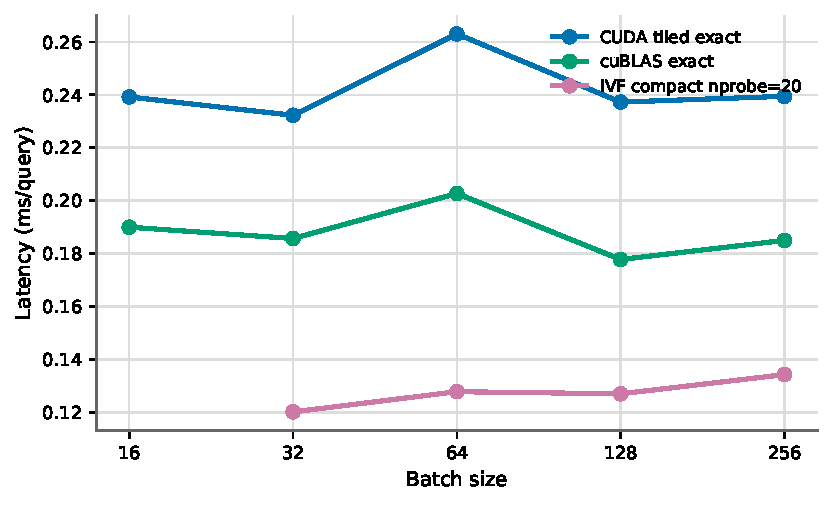
\includegraphics[width=\linewidth]{../files/figures/gpu_report/fig_gpu_03_batch.pdf}
    \caption{batch size 对 exact 与 IVF 的影响}
    \label{fig:batch-sensitivity}
\end{subfigure}
\hfill
\begin{subfigure}{0.49\linewidth}
    \centering
    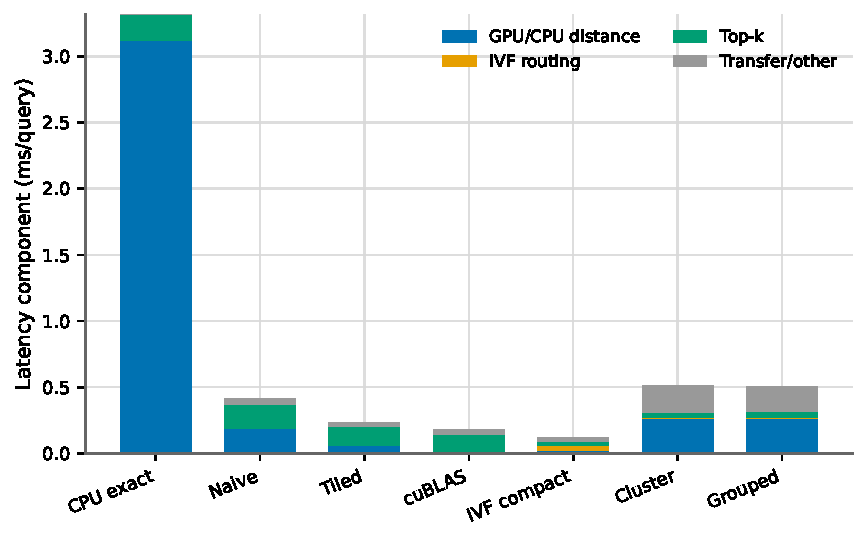
\includegraphics[width=\linewidth]{../files/figures/gpu_report/fig_gpu_04_breakdown.pdf}
    \caption{代表性方法的 query-time 拆分}
    \label{fig:stage-breakdown}
\end{subfigure}
\caption{矩阵路径与 IVF 路径的 batch 敏感性及阶段瓶颈。}
\label{fig:batch-breakdown}
\end{figure}

图~\ref{fig:batch-breakdown} 汇总了 batch size 与阶段拆分两类信息，其中图~\ref{fig:batch-sensitivity} 表明 batch size 并非越大越好。对 cuBLAS exact，batch=128 时延迟最低，batch=256 后 top-k 和分数矩阵搬运压力上升；对 IVF compact，batch=32 最优，batch 继续增大后 padding 到 batch 内最大候选数会增加无效距离计算，且 host 端 top-k 需要处理更大的临时数组。图~\ref{fig:stage-breakdown} 的阶段拆分也显示，CPU exact 的时间几乎全部消耗在距离计算；GPU exact 则转为 top-k 主导；IVF compact 的计算、routing、top-k 更均衡，因而总延迟最低。

\begin{table}[H]
\centering
\small
\caption{代表性路径的阶段拆分，单位为 \msq{}。}
\label{tab:stage-breakdown}
\begin{tabular}{lrrrrr}
\toprule
方法 & candidate/routing & distance compute & top-k & other & total \\
\midrule
CPU exact & 0.0000 & 3.1221 & 0.1933 & 0.0000 & 3.3154 \\
cuBLAS exact & 0.0000 & 0.0037 & 0.1388 & 0.0352 & 0.1778 \\
IVF compact & 0.0311 & 0.0258 & 0.0297 & 0.0335 & \textbf{0.1201} \\
\bottomrule
\end{tabular}
\end{table}

表~\ref{tab:stage-breakdown} 进一步揭示了三种路径的瓶颈迁移。CPU exact 中距离计算占 94\% 以上，说明 CPU 主要受 exact scan 吞吐限制；cuBLAS exact 的距离计算只占约 2\%，但 top-k 占 78\% 左右，说明 GPU 已经把内积问题基本解决，剩余瓶颈是完整分数矩阵带来的后处理；IVF compact 中 routing、distance 和 top-k 都在 0.03~\msq{} 量级，整体更加均衡。均衡并不意味着每个阶段都已经最优，而是说明单独优化任一阶段的收益有限，后续需要把候选生成、距离计算和 top-k 更紧密地融合，减少中间结果 materialization。

从体系结构角度看，cuBLAS exact 的计算阶段非常短，但它仍要产生并回传 100000 个分数。对于 top-100 查询，这些分数中 99.9\% 最终被丢弃。IVF compact 的优势来自提前裁剪：它只为约 10613 个候选计算分数，丢弃比例大幅下降。GPU 的高吞吐适合处理规则密集计算，但 ANN 查询的最终目标不是生成完整分数矩阵，而是尽快得到 top-100 编号。因此，算法层面的候选裁剪可以比单纯提升 kernel FLOPS 更有效。

\subsection{IVF 的精度--速度权衡}

\begin{figure}[H]
\centering
\figgpu{fig_gpu_02_ivf_nprobe}
\caption{IVF compact 在 batch=128 下的 $nprobe$ 消融。$nprobe$ 提高会增加候选数和延迟，同时提升 recall。}
\label{fig:ivf-nprobe}
\end{figure}

图~\ref{fig:ivf-nprobe} 显示 $nprobe$ 是 IVF 中最关键的精度--速度旋钮。$nprobe=12$ 时延迟只有 0.0940~\msq{}，但 recall@100=0.9105；$nprobe=16$ 为 0.1127~\msq{}、recall=0.9358，仍低于阈值；$nprobe=20$ 达到 recall=0.9510，是第一组满足阈值的配置。继续增加到 64、128 后 recall 分别提高到 0.9927、0.9989，但候选数从 10613 增至 28633、53611，延迟也升至 0.2598、0.5327~\msq{}。这一趋势符合 IVF 的复杂度模型：候选数近似随 $nprobe$ 线性增长，top-k 与 device--host 分数搬运也随候选数增长。

\begin{table}[H]
\centering
\small
\caption{IVF compact 在 batch=128 下的 $nprobe$ 消融。}
\label{tab:ivf-nprobe}
\begin{tabular}{rrrrr}
\toprule
$nprobe$ & recall@100 & latency(\msq) & avg candidates & waste ratio \\
\midrule
12  & 0.9105 & 0.0940 & 6911  & 1.890 \\
16  & 0.9358 & 0.1127 & 8829  & 1.743 \\
18  & 0.9439 & 0.1179 & 9723  & 1.679 \\
20  & 0.9510 & 0.1270 & 10613 & 1.630 \\
22  & 0.9569 & 0.1291 & 11523 & 1.597 \\
24  & 0.9614 & 0.1484 & 12384 & 1.560 \\
32  & 0.9748 & 0.1631 & 15808 & 1.460 \\
48  & 0.9872 & 0.2468 & 22379 & 1.407 \\
64  & 0.9927 & 0.2598 & 28633 & 1.338 \\
96  & 0.9973 & 0.4147 & 41114 & 1.279 \\
128 & 0.9989 & 0.5327 & 53611 & 1.229 \\
\bottomrule
\end{tabular}
\end{table}

表~\ref{tab:ivf-nprobe} 中 \texttt{waste\_ratio} 随 $nprobe$ 增大而下降，看似与 latency 增长相反。原因是 $nprobe$ 较小时，不同 query 的候选列表长度受簇大小波动影响更明显，batch padding 的相对比例较高；$nprobe$ 增大后，每个 query 覆盖更多簇，候选总数变大，长度差异在相对意义上被摊薄，因此 waste ratio 下降。但绝对候选数增长更快，导致 latency 仍持续上升。这说明不能只看 waste ratio，还要同时看 \texttt{avg\_candidates} 和 recall。最优配置需要在候选规模、padding 浪费和质量阈值三者之间取得平衡。

从算法角度看，$nprobe$ 增大对 recall 的边际收益递减。前几个被探测簇通常包含与 query 最相近的一组 centroid，对 top-100 的贡献最大；后续簇与 query 的相似度较低，带来的新增真近邻数量减少，却仍要付出完整候选距离计算成本。实验中 $nprobe=20$ 到 32 的 recall 增量约为 0.0237，latency 增量约为 0.0361~\msq{}；$nprobe=64$ 到 128 的 recall 增量只有 0.0062，latency 却增加约 0.2728~\msq{}。这体现了典型的 ANN 精度--速度边际成本上升。

\subsection{IVF 批处理浪费与分组策略}

\begin{figure}[H]
\centering
\figgpu{fig_gpu_05_waste}
\caption{不同 IVF 批处理方式的浪费计算比例。compact 路径只在 batch 内做候选 padding；按簇 baseline 会对不探测该簇的 query 也计算距离。}
\label{fig:ivf-waste}
\end{figure}

按簇矩阵 baseline 的问题在图~\ref{fig:ivf-waste} 中非常明显：当 $nprobe=22$ 时，有效候选数约 11268，但由于 batch 中不同 query 的探测簇集合不同，按簇计算需要约 8.78 倍的距离计算；compact 路径的 waste ratio 为 1.60，主要来自候选列表 padding。grouped 版本在 $nprobe=32$ 下把 latency 从 0.6802 降到 0.5213~\msq{}，但 waste ratio 几乎不变，说明简单按最近中心排序只能减少部分 kernel launch 和 host 端组织开销，不能显著改变多个 query 的完整 $nprobe$ 集合差异。更强的 grouping 需要根据 $nprobe$ 集合的 Jaccard 相似度或 centroid bitset 聚类 batch，但这会引入额外排序与调度成本，且 batch 越小越容易削弱 GPU 吞吐。

\begin{table}[H]
\centering
\small
\caption{IVF 批处理组织方式对照。}
\label{tab:ivf-organization-results}
\begin{tabular}{lrrrr}
\toprule
方法 & $nprobe$ & recall@100 & latency(\msq) & waste ratio \\
\midrule
compact & 16 & 0.9358 & 0.1127 & 1.743 \\
cluster baseline & 16 & 0.9294 & 0.4786 & 11.323 \\
grouped baseline & 16 & 0.9294 & 0.4904 & 11.362 \\
\midrule
compact & 22 & 0.9569 & 0.1291 & 1.597 \\
cluster baseline & 22 & 0.9513 & 0.5135 & 8.783 \\
grouped baseline & 22 & 0.9513 & 0.5089 & 8.785 \\
\midrule
compact & 32 & 0.9748 & 0.1631 & 1.460 \\
cluster baseline & 32 & 0.9708 & 0.6802 & 6.426 \\
grouped baseline & 32 & 0.9708 & 0.5213 & 6.438 \\
\bottomrule
\end{tabular}
\end{table}

表~\ref{tab:ivf-organization-results} 表明，cluster baseline 的性能低于 compact 并不意味着矩阵化思路本身不可行，而是说明 batch 组织必须与候选集合结构匹配。若所有 query 探测的簇高度重合，按簇矩阵乘会有较高效率；但实际 query 分布较分散，一个 batch 中出现的簇并集远大于单个 query 的 $nprobe$ 集合。此时簇级矩阵乘会把许多 query 与无关簇配对，形成数量级更高的 scored pairs。grouped 只按最近中心排序，对第 2 到第 $nprobe$ 个中心缺乏约束，因此无法显著降低簇集合并集大小。

候选一致性保证也影响实现复杂度。compact IVF 中每个 query 的候选列表由其 $nprobe$ 个簇直接拼接得到，score/id 数组按 query 独立组织，top-k 不会混入其他 query 的无关候选；因此一致性容易保证。cluster baseline 中，一个簇级 kernel 可能为 batch 内所有 query 产生分数，但其中只有部分 query 真正需要该簇，后处理必须根据 query--cluster membership 过滤，否则会把无效候选加入 top-k。这个过滤逻辑增加了 host 端复杂度，也解释了为什么它即使有规则矩阵形态，端到端表现仍然较差。

compact IVF 因此是当前实现中的更优折中：它放弃按簇矩阵的整齐形态，改为按 query 的真实候选列表计算，减少无效距离；代价是每个 batch 的候选长度仍需 padding，且 top-k 保持在 CPU 端。若进一步优化，可把候选 top-k 移到 GPU 端，并使用 block-level heap 或 bitonic selection 直接在 device 上输出 top-100，从而避免回传所有候选分数。

\section{性能建模与体系结构分析}

GPU ANN 的端到端时间可以近似拆成
\[
T = T_{\mathrm{route}} + T_{\mathrm{distance}} + T_{\mathrm{copy}} + T_{\mathrm{topk}} + T_{\mathrm{launch}},
\]
其中 routing 包括 query 到 centroid 的打分和候选列表构造，distance 是 GPU 端内积，copy 是候选分数和编号回传，top-k 是 host 端选择，launch 是 kernel 调度与同步成本。exact scan 中 $T_{\mathrm{route}}=0$，但 $T_{\mathrm{distance}}$ 和 $T_{\mathrm{copy}}$ 均与 $N$ 成正比；IVF 中额外引入 routing，却把 distance/copy/top-k 的规模从 $N$ 降低到平均候选数 $C(q)$。当 $C(q)\ll N$ 时，routing 的固定开销可以被候选裁剪收益抵消。

对 compact IVF，若 batch 内最大候选数为 $C_{\max}$，batch 大小为 $m$，实际执行的距离数为 $mC_{\max}$，有效距离数为 $\sum_{i=1}^{m} C_i$。浪费比为
\[
    \rho = \frac{mC_{\max}}{\sum_{i=1}^{m} C_i}.
\]
该公式解释了 batch size 的双重作用。增大 batch 可以提高 GPU occupancy、摊薄 launch 和固定开销；但它也更容易遇到极大候选列表，使 $C_{\max}$ 上升，并让更多 query 被 padding 到这个长度。batch=32 的最优结果说明，在当前 DEEP100K 分布下，中等 batch 能同时保持足够并行度和较低 padding。batch=128 虽然 GPU 吞吐更稳定，但浪费比上升，最终 latency 略高。

cache 行为方面，exact scan 的 base 矩阵按连续内存存储，query batch 也连续存储，cuBLAS 能充分利用 L2 cache、shared memory 和寄存器 blocking。compact IVF 的访问则更不规则：候选编号来自多个倒排簇，虽然每个簇内部向量连续，但一个 query 的候选列表由多个簇拼接，跨 query 的候选位置也不一定相邻。因此 compact kernel 的 raw FLOPS 不可能接近 SGEMM。它胜出的原因不是单次内积更快，而是把内积数量减少到约 10.6\%。这也是 ANN 与普通 dense linear algebra 的关键差异：算法层面的候选裁剪通常比单个 kernel 的峰值吞吐更重要。

top-k 是当前实现的主要后续优化方向。CPU heap top-k 对每个 query 的复杂度约为 $O(C\log k)$，其中 $C$ 是候选数、$k=100$。exact scan 的 $C=100000$，top-k 因而占据主导；compact IVF 的 $C\approx10613$，top-k 降到 0.0297~\msq{}，但仍与 distance compute 同量级。device 端 top-k 可以减少分数回传量，不过它需要分层选择、线程间同步和临时缓冲；在候选数不大时，额外 kernel launch 可能抵消收益。

\begin{table}[H]
\centering
\small
\caption{后续优化方向的收益来源与潜在风险。}
\label{tab:future-work}
\begin{tabular}{p{0.22\linewidth}p{0.33\linewidth}p{0.33\linewidth}}
\toprule
优化方向 & 预期收益 & 风险与复杂度 \\
\midrule
GPU 端 top-k & 减少候选分数回传，只输出 top-100；降低 host top-k 时间 & 需要分层选择算法和额外临时缓冲；小候选数下 launch 开销可能过高 \\
prefix-sum 候选压缩 & 避免 batch padding，理论上把 waste ratio 接近 1 & 需要 device 端候选偏移生成和变长列表调度，kernel 更复杂 \\
Jaccard/bitset grouping & 提高 batch 内 $nprobe$ 集合重合度，降低簇级 baseline 浪费 & 排序和分组本身有开销，且可能破坏输入 query 顺序与缓存局部性 \\
PQ/OPQ 压缩 & 降低距离计算维度和内存带宽需求 & 需要额外训练、查表距离和重排；recall 调参空间更大 \\
HIP/rocBLAS 移植 & 复用 CUDA 思路到 AMD GPU，扩展平台覆盖 & wavefront 大小、库性能和编译工具链不同，需要重新调参 \\
\bottomrule
\end{tabular}
\end{table}
表~\ref{tab:future-work} 将后续优化按收益来源和复杂度拆开，避免只给出单一方向而忽略实现风险。

从任务划分角度看，GPU exact scan 是规则的水平划分，每个线程块负责分数矩阵的一部分，query 之间没有写冲突；IVF compact 是候选列表划分，每个 query 只计算自己的候选集合，需要保证候选编号、score buffer 和 top-k 输入一一对应；按簇 baseline 则是簇级垂直划分，矩阵形态更规则，但必须过滤不属于当前 query 的簇分数。实验结果说明，当前数据分布下减少无效候选比维持簇级矩阵形态更重要。

线程管理成本在 GPU 上主要表现为 launch 和同步。exact cuBLAS 用少量大 kernel 摊薄 launch 开销；cluster baseline 会产生较多小粒度簇级调度；compact IVF 用 batch kernel 覆盖 query--candidate 对，因此在 launch 次数和候选有效性之间取得更好的折中。

\section{实验边界与可移植性说明}

HIP 基础学习和 GPU ANN 实验处在两个层次。前者面向 GPU 编程模型本身，重点是线程索引、访存、atomic、归约和迭代程序结构；后者面向具体 ANN 查询任务，重点是 batch 距离计算、候选裁剪和 top-k 后处理的速度--精度权衡。两部分的联系主要体现在通用 GPU 编程概念上，HIP 题目解答见附录~\ref{app:hip-answers}。

进阶实验选择本地 NVIDIA CUDA 平台，是因为当前机器提供 GeForce RTX 4060 Laptop GPU 和成熟的 cuBLAS baseline。若迁移到 AMD/HIP 平台，host/device 内存管理和 kernel launch 流程可以保持相似结构，但 wavefront 大小、LDS 容量、编译器优化策略、rocBLAS kernel 行为以及最优 block size、batch size、候选 padding 都需要重新测量。本文的性能结论因此只对当前数据集、当前 GPU 和当前实现成立；迁移时应沿用参数 sweep 和阶段拆分方法重新搜索配置。

\section{结论}

GPU ANN 的有效加速依赖两个条件：距离计算必须以 batch 形式形成足够大的并行工作量，候选集合又必须足够小，使分数回传和 top-k 不压过 GPU 计算收益。本文的 exact 矩阵乘法路线验证了 GPU 对大规模内积的优势，其中 cuBLAS exact 达到 0.1778~\msq{}；IVF compact 进一步用候选裁剪换取更低延迟，在 recall@100$\ge0.95$ 下达到 0.1201~\msq{}。按簇 IVF baseline 展示了批处理中簇集合不一致导致的浪费，简单 grouping 只能部分缓解 launch 和组织开销，不能替代候选压缩。整体来看，最优策略不是单纯扩大 batch 或追求 exact recall，而是在阈值 recall 附近选择最小 $nprobe$，并控制 batch padding、top-k 与传输开销。



\clearpage
\appendix

\section{HIP Notebook 题目与答案汇总}
\label{app:hip-answers}

本附录整理 HIP 六个基础实验中的题目与填写结果。每个小节先给出题目要求，再给出对应答案。

\subsection{Lab 1: Vector Addition}

\subsubsection{线程索引计算}
\noindent\textbf{题目：} 1D grid 与 1D block 中，全局线程索引为
\[
\mathrm{globalIdx}=\mathrm{blockIdx.x}\times\mathrm{blockDim.x}+\mathrm{threadIdx.x}.
\]
根据下表填写每个线程的全局索引。
\begin{center}
\small
\begin{tabular}{rrrr}
\toprule
\texttt{blockIdx.x} & \texttt{blockDim.x} & \texttt{threadIdx.x} & 全局索引 \\
\midrule
0 & 256 & 100 & \underline{\hspace{2.5em}} \\
2 & 128 & 50 & \underline{\hspace{2.5em}} \\
5 & 64 & 0 & \underline{\hspace{2.5em}} \\
\bottomrule
\end{tabular}
\end{center}
\noindent\textbf{答案：}
\begin{center}
\small
\begin{tabular}{rl}
\toprule
序号 & 计算过程 \\
\midrule
1 & $0\times256+100=100$ \\
2 & $2\times128+50=306$ \\
3 & $5\times64+0=320$ \\
\bottomrule
\end{tabular}
\end{center}

\subsubsection{Exercise 1: GPU Specifications}
\noindent\textbf{题目：} 根据设备信息填写 GPU 规格，并计算所有 CU 充分利用时可同时执行的线程数。
\begin{center}
\small
\begin{tabular}{p{0.28\linewidth}p{0.30\linewidth}p{0.32\linewidth}}
\toprule
属性 & 待填写值 & 含义 \\
\midrule
Device Name & \underline{\hspace{6em}} & GPU 型号标识 \\
Compute Units & \underline{\hspace{6em}} & 并行执行单元数量 \\
Wavefront Size & \underline{\hspace{6em}} & 每个 wavefront 的线程数 \\
Max Threads per Block & \underline{\hspace{6em}} & \texttt{blockDim} 上限 \\
Max Shared Memory per Block & \underline{\hspace{6em}} & 每个 block 可用 LDS \\
\bottomrule
\end{tabular}
\end{center}
\noindent\textbf{答案：}
\begin{center}
\small
\begin{tabular}{ll}
\toprule
属性 & 填写结果 \\
\midrule
Device Name & AMD Radeon 890M Graphics \\
Compute Units & HIP 报告 8 个 CU，\texttt{rocminfo} 显示 16 个 CU \\
Wavefront Size & 32 \\
Max Threads per Block & 1024 \\
Max Shared Memory per Block & 64 KB，即 65536 bytes \\
\bottomrule
\end{tabular}
\end{center}
若按 HIP 报告的 8 个 CU、每 CU 64 个 wavefront、每 wavefront 32 个线程计算，则
\[
8\times64\times32=16384
\]
个线程可同时处于活跃 wavefront 中。

\subsubsection{Exercise 2: Implement the Kernel}
\noindent\textbf{题目：} 完成向量加法 kernel 中的全局索引、边界判断和计算语句。
\begin{lstlisting}[language=C++]
__global__ void vector_add(const float* A, const float* B, float* C, int N) {
    int idx = _______________________________;
    if (______) {
        C[idx] = _______________________________;
    }
}
\end{lstlisting}
\noindent\textbf{答案：}
\begin{lstlisting}[language=C++]
int idx = blockIdx.x * blockDim.x + threadIdx.x;
if (idx < N) {
    C[idx] = A[idx] + B[idx];
}
\end{lstlisting}
这里的边界检查用于处理 $N$ 不能被 block size 整除时最后一个 block 中的空闲线程。

\subsubsection{Exercise 3: Launch Configuration Calculation}
\noindent\textbf{题目：} 给定 $N=1000$，填写不同 block size 下的 grid size、总线程数和空闲线程数，并回答哪个 block size 的线程利用率最高。
\begin{center}
\small
\begin{tabular}{rrrr}
\toprule
Block Size & Grid Size & Total Threads & Idle Threads \\
\midrule
64 & \underline{\hspace{2.5em}} & \underline{\hspace{2.5em}} & \underline{\hspace{2.5em}} \\
128 & \underline{\hspace{2.5em}} & \underline{\hspace{2.5em}} & \underline{\hspace{2.5em}} \\
256 & \underline{\hspace{2.5em}} & \underline{\hspace{2.5em}} & \underline{\hspace{2.5em}} \\
512 & \underline{\hspace{2.5em}} & \underline{\hspace{2.5em}} & \underline{\hspace{2.5em}} \\
\bottomrule
\end{tabular}
\end{center}
\noindent\textbf{答案：}
\begin{center}
\small
\begin{tabular}{rrrr}
\toprule
Block Size & Grid Size & Total Threads & Idle Threads \\
\midrule
64 & 16 & 1024 & 24 \\
128 & 8 & 1024 & 24 \\
256 & 4 & 1024 & 24 \\
512 & 2 & 1024 & 24 \\
\bottomrule
\end{tabular}
\end{center}
四种配置的线程利用率相同，均为 $1000/1024=97.66\%$。但实际性能还取决于 wavefront 对齐、occupancy、寄存器压力、shared memory 使用量和调度开销，因此线程利用率最高并不必然等于性能最高。

\subsubsection{Exercise 4: Analyze Your Results}
\noindent\textbf{题目：} 根据多次运行结果回答：最低平均执行时间对应的 block size、最高内存带宽对应的 block size、差异是否统计显著，以及为什么 Vector Add 更依赖带宽而不是 block size。

\noindent\textbf{答案：}
\begin{enumerate}[label=\arabic*.]
\item 最低平均执行时间对应 512 threads per block，平均时间为 $0.1412\,\mathrm{ms}$。
\item 因为总传输字节数固定，执行时间最低时带宽最高，所以最高内存带宽也对应 512 threads per block。
\item 差异不强。各 block size 的均值接近，多数误差范围有重叠。
\item Vector Add 每个元素只做一次加法，却需要读取两个全局内存数组并写回一个输出数组，因此主要受 global memory bandwidth 限制，而不是算术吞吐限制。
\end{enumerate}

\subsubsection{Exercise 5: Wavefront Analysis}
\noindent\textbf{题目：} block size 为 100 时，分别在 wave32 和 wave64 模式下计算每个 block 需要的 wavefront 数和浪费 lane 数；并解释 wavefront 内部分支不一致时会发生什么。

\noindent\textbf{答案：}
\begin{center}
\small
\begin{tabular}{lrr}
\toprule
模式 & Wavefronts per block & Wasted lanes \\
\midrule
wave32 & $\lceil100/32\rceil=4$ & $4\times32-100=28$ \\
wave64 & $\lceil100/64\rceil=2$ & $2\times64-100=28$ \\
\bottomrule
\end{tabular}
\end{center}
同一 wavefront 内线程走不同分支时，GPU 会用掩码分别执行不同分支路径，实际表现为分支路径串行化。这会降低并行效率，即通常所说的 branch divergence。

\subsubsection{Exercise 6: Occupancy Calculation}
\noindent\textbf{题目：} 对 Radeon 8060S/RDNA 3.5，假设 wavefront size 为 32、每 CU 最大 64 个 active wavefront，填写不同 block size 下可驻留 block 数和 active wavefront 数。

\noindent\textbf{答案：}
\begin{center}
\small
\begin{tabular}{rlll}
\toprule
Block Size & Blocks that fit & Active Wavefronts & 说明 \\
\midrule
32 & 受最大 block 数限制，为 64 & 64 & 达到 64 wavefront/CU 上限 \\
64 & 32 & 64 & 受最大 active wavefront 限制 \\
128 & 16 & 64 & 受最大 active wavefront 限制 \\
256 & 8 & 64 & 受最大 active wavefront 限制 \\
512 & 4 & 64 & 受最大 active wavefront 限制 \\
1024 & 2 & 64 & 受最大 active wavefront 限制 \\
\bottomrule
\end{tabular}
\end{center}
这些结果是在没有额外寄存器和 LDS 限制时的理论 occupancy。实际 kernel 还可能受到寄存器数量、shared memory、指令混合和访存模式影响。

\subsubsection{Exercise 7: Analyze Sub-Wavefront Results}
\noindent\textbf{题目：} 根据多次运行结果填写 block size 8、16、32、256 的平均时间，判断 sub-wavefront block size 是否有明显性能损失，并说明若换到 MI100/wave64 哪些 block size 会成为 sub-wavefront。

\noindent\textbf{答案：}
\begin{center}
\small
\begin{tabular}{rr}
\toprule
Block Size & Mean Time \\
\midrule
8 & $0.1943\,\mathrm{ms}$ \\
16 & $0.1467\,\mathrm{ms}$ \\
32 & $0.1480\,\mathrm{ms}$ \\
256 & $0.1469\,\mathrm{ms}$ \\
\bottomrule
\end{tabular}
\end{center}
block size 8 有明显损失，因为它只使用 wave32 的一部分 lane，却仍占用一个完整 wavefront 的调度资源。block size 16 在该次测量中接近 wave-aligned 配置，损失不明显。若在 MI100 的 wave64 模式下，8、16、32 都会成为 sub-wavefront block size。

\subsubsection{Challenge Exercise: Grid-stride Loop}
\noindent\textbf{题目：} 修改 kernel，使每个线程可处理多个元素。需要填写总线程数 stride，并说明它相比一线程一元素映射的优势。
\begin{lstlisting}[language=C++]
__global__ void vector_add_multi(const float* A, const float* B, float* C,
                                  int N, int elements_per_thread) {
    int tid = blockIdx.x * blockDim.x + threadIdx.x;
    int stride = _______________________________;
    for (int i = tid; i < N; i += stride) {
        C[i] = A[i] + B[i];
    }
}
\end{lstlisting}
\noindent\textbf{答案：}
\begin{lstlisting}[language=C++]
int stride = gridDim.x * blockDim.x;
\end{lstlisting}
grid-stride loop 允许固定数量的线程覆盖任意长度数组，使 kernel 不必为超大输入启动极大的 grid，同时每个线程可处理多个元素，提高 launch 开销摊销效果。

\subsection{Lab 2: Matrix Transpose}

\subsubsection{Exercise 1: 2D Indexing}
\noindent\textbf{题目：} 给定 \texttt{blockDim=(32,32)}，计算二维全局索引；并计算 $rows=100, cols=200$ 的矩阵需要多少个 block。
\begin{center}
\small
\begin{tabular}{lll}
\toprule
\texttt{blockIdx} & \texttt{threadIdx} & Global $(idx,idy)$ \\
\midrule
(0,0) & (5,10) & $(\underline{\hspace{2em}},\underline{\hspace{2em}})$ \\
(1,0) & (0,0) & $(\underline{\hspace{2em}},\underline{\hspace{2em}})$ \\
(2,3) & (15,20) & $(\underline{\hspace{2em}},\underline{\hspace{2em}})$ \\
\bottomrule
\end{tabular}
\end{center}
\noindent\textbf{答案：}
\begin{center}
\small
\begin{tabular}{lll}
\toprule
\texttt{blockIdx} & \texttt{threadIdx} & Global $(idx,idy)$ \\
\midrule
(0,0) & (5,10) & (5,10) \\
(1,0) & (0,0) & (32,0) \\
(2,3) & (15,20) & (79,116) \\
\bottomrule
\end{tabular}
\end{center}
对 $rows=100,cols=200$，$grid_x=\lceil200/32\rceil=7$，$grid_y=\lceil100/32\rceil=4$，因此共需 $7\times4=28$ 个 block。

\subsubsection{Exercise 2: Understand the Index Transformation}
\noindent\textbf{题目：} 对 $4\times6$ 矩阵填写指定线程的输入下标和转置输出下标，并解释为什么写入公式是 \texttt{idx * rows + idy}。

\noindent\textbf{答案：}
\begin{center}
\small
\begin{tabular}{lll}
\toprule
Thread $(idx,idy)$ & Input Index & Output Index \\
\midrule
(1,0) & $0\times6+1=1$ & $1\times4+0=4$ \\
(0,1) & $1\times6+0=6$ & $0\times4+1=1$ \\
(3,2) & $2\times6+3=15$ & $3\times4+2=14$ \\
\bottomrule
\end{tabular}
\end{center}
转置后输出矩阵尺寸为 $cols\times rows$，输出矩阵每行长度为 $rows$。原矩阵列号 $idx$ 变成输出行号，原矩阵行号 $idy$ 变成输出列号，因此 row-major 输出下标为 $idx\times rows+idy$。

\subsubsection{Exercise 3: Performance Analysis}
\noindent\textbf{题目：} 记录四组矩阵转置测试的执行时间，并分析大测试元素数约为 test 2 的 500 倍时，耗时是否也增长 500 倍。

\noindent\textbf{答案：}
\begin{center}
\small
\begin{tabular}{rrr}
\toprule
Test & Dimensions / Elements & Time \\
\midrule
1 & $16\times16$ / 256 & $0.0072\,\mathrm{ms}$ \\
2 & $128\times32$ / 4096 & $0.0100\,\mathrm{ms}$ \\
3 & $1\times1024$ / 1024 & $0.0081\,\mathrm{ms}$ \\
4 & $1001\times2001$ / 2003001 & $0.2428\,\mathrm{ms}$ \\
\bottomrule
\end{tabular}
\end{center}
不是线性增长。大测试元素数约为 $2003001/4096\approx489$ 倍，但执行时间仅约为 $0.2428/0.0100=24.3$ 倍。小测试受 kernel launch、occupancy 不足等固定开销影响更明显；大测试更能体现实际内存访问行为，但 naive transpose 仍受非合并写限制。

\subsubsection{Exercise 4: Coalescing Analysis}
\noindent\textbf{题目：} 对 $1024\times1024$ 矩阵和 $32\times32$ block，分析读取 \texttt{input[idy * cols + idx]} 是否合并访问、写入 \texttt{output[idx * rows + idy]} 的 stride，以及 32 个线程非合并写需要多少个 128-byte transaction。

\noindent\textbf{答案：}
\begin{enumerate}[label=\arabic*.]
\item 对固定 $idy$，连续 $idx$ 读取连续 float 地址，因此读取是 coalesced。
\item 写入 stride 为 $rows$ 个 float。对 $1024\times1024$ 矩阵，连续线程写地址相隔 $1024$ 个 float，即 $4096$ bytes。
\item 需要 32 个 transaction。每个线程写入不同的 128-byte 区域，wavefront 无法把这些写合并为一次 transaction。
\end{enumerate}

\subsubsection{Exercise 5: Tiled Transpose Analysis}
\noindent\textbf{题目：} 解释 tiled transpose 中 \texttt{tile[BLOCK\_SIZE][BLOCK\_SIZE+1]} 的 $+1$、写回阶段交换 \texttt{blockIdx.x} 和 \texttt{blockIdx.y} 的原因，并计算 \texttt{BLOCK\_SIZE=32} 时每个 block 的 shared memory 用量。

\noindent\textbf{答案：}
\begin{enumerate}[label=\arabic*.]
\item $+1$ 使 shared memory 每行 stride 从 32 个 float 变为 33 个 float，转置访问 tile 时可减少多个线程落到同一 bank 的冲突。
\item 转置会交换行列。输入 tile 位于 $(blockIdx.x,blockIdx.y)$，输出 tile 应写到 $(blockIdx.y,blockIdx.x)$；交换 block 索引可把 tile 放到正确转置位置，并让写回按行主序合并访问。
\item shared memory 用量为 $32\times(32+1)\times4=4224$ bytes。
\end{enumerate}

\subsection{Lab 3: Histogram}

\subsubsection{Exercise 1: Analyze the Problem}
\noindent\textbf{题目：} naive histogram 中每个 block 负责一个 bin，每个 block 扫描完整输入。回答每个元素被读取多少次；当 $num\_bins=256,N=10M$ 时总 global memory traffic；以及该方法为何低效。

\noindent\textbf{答案：}
\begin{enumerate}[label=\arabic*.]
\item 每个输入元素会被读取 $num\_bins$ 次，因为每个 bin 对应一个 block，每个 block 都扫描完整输入。
\item 读取次数为 $N\times num\_bins=10000000\times256=2560000000$ 次 integer read。每个 integer 为 4 bytes，因此流量为 $10240000000$ bytes，约 $10.24$ GB。
\item 工作量和内存流量按 $O(N\times num\_bins)$ 增长，而不是 $O(N)$。绝大多数读取不会为当前 bin 产生贡献，重复 global memory 读取成为主要瓶颈。
\end{enumerate}

\subsubsection{Exercise 2: Understand the Optimization}
\noindent\textbf{题目：} 解释 shared memory 上的 \texttt{atomicAdd} 为什么比 global memory 更快；merge 阶段每个 bin 有多少 global atomic；以及 grid-stride loop 的作用。

\noindent\textbf{答案：}
\begin{enumerate}[label=\arabic*.]
\item shared memory 位于片上 LDS，延迟更低、带宽更高；atomic 冲突被限制在一个 block 内。global memory atomic 会跨整个 grid 争用，并触发更慢的片外内存操作。
\item 每个 block 对每个 bin 执行一次 global \texttt{atomicAdd}。block 内先构造 shared-memory 局部直方图，再把每个 bin 的局部计数合并到全局直方图。
\item grid-stride loop 让固定数量线程覆盖任意长度输入。线程按总线程数为 stride 处理多个元素，确保每个输入元素只从 global memory 读取一次。
\end{enumerate}

\subsubsection{Exercise 3: Record Results}
\noindent\textbf{题目：} 填写 serial CPU、naive GPU 和 optimized GPU 在 testcase 2、testcase 4 上的执行时间，并计算 optimized 相对 serial/naive 的加速比。

\noindent\textbf{答案：}
\begin{center}
\small
\begin{tabular}{lrr}
\toprule
Implementation & Time(testcase 2) & Time(testcase 4) \\
\midrule
Serial CPU & $2.5611\,\mathrm{ms}$ & $22.8836\,\mathrm{ms}$ \\
Naive GPU & $15.0112\,\mathrm{ms}$ & $2549.3780\,\mathrm{ms}$ \\
Optimized GPU & $0.4570\,\mathrm{ms}$ & $4.4452\,\mathrm{ms}$ \\
\bottomrule
\end{tabular}
\end{center}
Optimized vs Serial：testcase 2 为 $2.5611/0.4570=5.60\times$，testcase 4 为 $22.8836/4.4452=5.15\times$。Optimized vs Naive：testcase 2 为 $15.0112/0.4570=32.85\times$，testcase 4 为 $2549.3780/4.4452=573.50\times$。

\subsubsection{Exercise 4: Memory Efficiency}
\noindent\textbf{题目：} 计算 optimized histogram 相比 naive histogram 的 global input read 降低比例：
\[
\mathrm{Reduction}=\frac{N\times num\_bins}{N}.
\]
\noindent\textbf{答案：} 降低比例为 $num\_bins$。例如 256 个 bin 时，optimized 方法把 global input read 降低 $256\times$；64 个 bin 时降低 $64\times$。

\subsubsection{Exercise 5: Contention Scenarios}
\noindent\textbf{题目：} 分析两种输入分布下的 atomic contention：所有输入值相同，以及输入值在所有 bin 上均匀分布。

\noindent\textbf{答案：}
\begin{enumerate}[label=\arabic*.]
\item 所有输入值相同时性能会变慢。测量中 all-same 数据耗时 $0.6802\,\mathrm{ms}$，uniform 数据耗时 $0.4543\,\mathrm{ms}$。原因是所有线程更新同一个 bin，atomic 操作严重串行化。optimized kernel 中冲突发生在 shared memory，比 global contention 便宜，但仍是最差分布。
\item 均匀分布时 contention 较低。更新被分散到多个 bin，同一 block 或 wavefront 内同时更新同一 shared-memory 地址的线程更少。
\end{enumerate}

\subsection{Lab 4: Reduction}

\subsubsection{Exercise 1: Understand Tree Reduction}
\noindent\textbf{题目：} 对 1024 个元素、block size 256 的树形归约，计算每个 block 内归约步数、block-level reduction 后剩余 partial sums 数量，并解释每步后使用 \texttt{\_\_syncthreads()} 的原因。

\noindent\textbf{答案：}
\begin{enumerate}[label=\arabic*.]
\item 每个 block 归约 256 个元素，需要 $\log_2(256)=8$ 步，stride 依次为 128、64、32、16、8、4、2、1。
\item $\lceil1024/256\rceil=4$，因此剩余 4 个 partial sums。
\item 每一步中后续线程会读取前一步其他线程写入的 shared memory 值。\texttt{\_\_syncthreads()} 保证所有写入完成后再进入下一步读取，避免读到未更新数据。
\end{enumerate}

\subsubsection{Exercise 2: Analyze Occupancy Results}
\noindent\textbf{题目：} 根据测试输出填写 block size、warps per block、occupancy 和执行时间，并回答更高 occupancy 是否总意味着更好性能。

\noindent\textbf{答案：}
\begin{center}
\small
\begin{tabular}{rrrr}
\toprule
Block Size & Warps/Block & Occupancy & Execution Time \\
\midrule
64 & 2 & 100\% & 未在当前输出报告 \\
128 & 4 & 100\% & 未在当前输出报告 \\
256 & 8 & 100\% & Tree/shared memory 为 $0.0632\,\mathrm{ms}$ \\
512 & 16 & 100\% & 未在当前输出报告 \\
1024 & 32 & 100\% & 未在当前输出报告 \\
\bottomrule
\end{tabular}
\end{center}
这些 occupancy 值假设 wave32 执行，且没有额外寄存器或 shared memory 限制。更高 occupancy 不一定带来更好性能；reduction 还取决于访存合并、同步开销、atomic contention、block 数量以及每个线程的有效工作量。

\subsubsection{Exercise 3: Think About Trade-offs}
\noindent\textbf{题目：} 对 $N=1M$，计算 block size 64 和 1024 时最终 global atomic 数量，并解释较少 atomic 为什么可能提高性能。

\noindent\textbf{答案：}
\begin{enumerate}[label=\arabic*.]
\item block size 64 时，$grid\_size=\lceil1000000/64\rceil=15625$，因此有 15625 次最终 global atomic。
\item block size 1024 时，$grid\_size=\lceil1000000/1024\rceil=977$，因此有 977 次最终 global atomic。
\item 每个 block 最终对全局输出做一次 \texttt{atomicAdd}。block 数越少，global atomic 越少，对单一输出地址的争用和全局同步开销也越低。
\end{enumerate}

\subsubsection{Exercise 4: Algorithm Analysis}
\noindent\textbf{题目：} 分析树形归约第一步后空闲线程比例；解释 warp shuffle 为什么不需要 \texttt{\_\_syncthreads()}；说明 multi-element per thread 如何提升内存带宽利用。

\noindent\textbf{答案：}
\begin{enumerate}[label=\arabic*.]
\item 第一轮后有一半线程空闲。例如 256 线程 block 中，第一步后只有 128 个线程继续参与归约。
\item warp shuffle 在同一 warp 或 wavefront 内交换寄存器值。同一 wavefront 的 lane lockstep 执行，不需要通过 shared memory 做 block-wide 同步。
\item 每个线程先在寄存器中读取并累加多个元素，再进入 shared-memory reduction。这样增加了每个线程的有效工作量，减少 block 数和最终 global atomic 数，并摊销 launch 与同步开销。
\end{enumerate}

\subsection{Lab 5: Monte Carlo Integration}

\subsubsection{Exercise 1: Understand the Algorithm}
\noindent\textbf{题目：} 解释为什么简单 atomic 版本在每个线程中除以 \texttt{n\_samples}；分析 atomic reduction 方法的时间复杂度；并说明如何改成 shared memory reduction。

\noindent\textbf{答案：}
\begin{enumerate}[label=\arabic*.]
\item 简单 atomic 实现中，每个线程直接计算最终贡献 $(b-a)y_i/n_{samples}$ 并累加到输出，因此输出已经是积分值。数学上它等价于先求和所有 $y_i$ 再统一乘 $(b-a)/n_{samples}$。优化版应在归约后再缩放，避免每个线程重复做除法。
\item kernel 启动 $O(n_{samples})$ 个工作，并执行 $O(n_{samples})$ 次 atomic add。由于所有 atomic 都更新同一个全局结果，atomic 阶段有严重争用，实际常数开销很高。
\item 每个 block 可先把样本值累加到 shared memory，再在 block 内树形归约。block-level sum 完成后，仅 thread 0 对全局结果执行一次 \texttt{atomicAdd}，把 global atomic 数从每样本一次降为每 block 一次。
\end{enumerate}

\subsubsection{Exercise 2: Manual Calculation}
\noindent\textbf{题目：} 对 test 1 手工验证积分结果。给定 $a=0,b=2,n=8$，公式为
\[
\mathrm{result}=\frac{b-a}{n}\sum_{i=1}^{n}y_i=\frac{2}{8}\sum y_i.
\]
填写 $y$ 值总和、期望结果，并判断是否与程序输出一致。

\noindent\textbf{答案：}
\[
\sum y_i=4.1805+1.7864+4.7554+3.9983+2.2786+1.1873+4.1222+1.442=23.7507.
\]
因此
\[
\frac{2}{8}\times23.7507=5.937675.
\]
该结果与程序输出 $5.937675$ 一致。

\subsubsection{Exercise 3: Scalability Analysis}
\noindent\textbf{题目：} 记录 sample count 为 100000、10000000、100000000 时的执行时间，分析 sample count 从 test 4 到 test 7 增加 100 倍时，执行时间增长多少以及是否线性。

\noindent\textbf{答案：}
\begin{center}
\small
\begin{tabular}{rrr}
\toprule
Test & Sample Count & Execution Time \\
\midrule
4 & 100000 & $0.095\,\mathrm{s}$ \\
7 & 10000000 & $0.983\,\mathrm{s}$ \\
8 & 100000000 & $8.455\,\mathrm{s}$ \\
\bottomrule
\end{tabular}
\end{center}
从 test 4 到 test 7，执行时间增长约 $0.983/0.095=10.35\times$，不是线性增长。小规模测试受进程启动、文件 I/O、GPU 初始化、内存分配和数据拷贝等固定开销影响更大；大规模测试中 GPU 并行度、内存带宽和 atomic contention 才成为主导因素。

\subsubsection{Exercise 4: Bottleneck Analysis}
\noindent\textbf{题目：} 若每个线程计算需要 1 cycle，global atomic 需要 100 cycles，计算 $N=1M$ 时理论效率；说明 shared memory reduction 如何改善；并计算 256 threads per block 下需要多少 global atomics。

\noindent\textbf{答案：}
\begin{enumerate}[label=\arabic*.]
\item 总 cycles 为
\[
1000000\times(1+100)=101000000.
\]
有用计算为 $1000000$ cycles，因此理论效率为
\[
\frac{1000000}{101000000}=0.0099,
\]
约 $0.99\%$。
\item shared memory reduction 在 block 内用片上内存完成局部求和，再由每个 block 执行一次 global atomic。它把数百万次争用严重的 global atomic 替换为数千次 global atomic 和较便宜的 block-local reduction。
\item $\lceil1000000/256\rceil=3907$ 个 block，因此需要 3907 次 global atomic。
\end{enumerate}

\subsubsection{Exercise 5: Precision Considerations}
\noindent\textbf{题目：} 回答 double precision 提供多少有效十进制位；若在 $N=100M$ 样本下改用 float，可能出现哪些问题。

\noindent\textbf{答案：}
\begin{enumerate}[label=\arabic*.]
\item double precision 提供约 15 到 17 位十进制有效数字，尾数为 53 bit。
\item float precision 只有约 6 到 7 位十进制有效数字。对 100M 样本，大量小贡献累加到较大 sum 上时可能被舍入掉，导致更大的数值误差；并行 atomic 的非确定累加顺序也会使结果更敏感。
\end{enumerate}

\subsubsection{Exercise 6: Optimization Analysis}
\noindent\textbf{题目：} 在优化版中，$N=1M$ 且使用 256 blocks 时 global atomic 数量是多少；grid-stride loop 的作用是什么；为什么只由 thread 0 执行 $(b-a)/n_{samples}$ 缩放。

\noindent\textbf{答案：}
\begin{enumerate}[label=\arabic*.]
\item 共有 256 次 global atomic，因为每个 block 在 shared-memory reduction 后只执行一次 \texttt{atomicAdd}。
\item grid-stride loop 让固定数量线程处理任意数量样本。每个线程按 $blockDim.x\times gridDim.x$ 为 stride 处理多个样本，提高覆盖能力并增加每线程有效工作。
\item block 内先把原始 $y$ 值归约成一个 partial sum，只有 thread 0 持有最终 block sum。在 thread 0 缩放可避免每个样本重复乘除同一常数，降低算术开销。
\end{enumerate}

\subsection{Lab 6: K-Means Clustering}

\subsubsection{Exercise 1: Algorithm Analysis}
\noindent\textbf{题目：} 分析 assignment kernel 中 $k=100$ 时每个线程的时间复杂度；解释 recalculation kernel 为什么先用 shared memory atomics 再用 global atomics；说明 centroid 没有点被分配时如何处理。

\noindent\textbf{答案：}
\begin{enumerate}[label=\arabic*.]
\item 每个线程处理一个点，并与全部 100 个 centroid 比较，因此每线程复杂度为 $O(k)=O(100)$，具体为 100 次距离计算。
\item shared memory atomics 更快，并把冲突限制在一个 block 内。每个 block 先在 shared memory 中累加局部 sum/count，再用少量 global atomic 合并，可降低 global atomic contention 和全局内存流量。
\item finalize kernel 检查 \texttt{count > 0}。若 count 为 0，则把上一轮 centroid 坐标复制到新 centroid 缓冲区，保持原 centroid 位置，避免除零。
\end{enumerate}

\subsubsection{Exercise 2: Performance Analysis}
\noindent\textbf{题目：} 记录 test 4 的执行时间：sample size 为 50000，clusters $k=50$，max iterations 为 100；并说明每次迭代中的主导计算。

\noindent\textbf{答案：} test 4 的实验输出为 $0.143\,\mathrm{s}$ real time。主导计算是 assignment phase：每个点都要计算到所有 centroid 的距离，每轮复杂度为 $O(Nk)$。update phase 主要是 $O(N)$ 的累加和 $O(k)$ 的最终 centroid 更新。

\subsubsection{Exercise 3: Compute Intensity}
\noindent\textbf{题目：} 对 $N=50000,k=50$，填写 assignment kernel 中每点距离计算次数、总距离计算次数；以及 update kernel 中 shared memory atomic 和 256 threads per block 时 global atomic 数量。

\noindent\textbf{答案：}
\begin{center}
\small
\begin{tabular}{ll}
\toprule
项目 & 结果 \\
\midrule
Assignment: distance calculations per point & 50 \\
Assignment: total distance calculations & $50000\times50=2500000$ \\
Update: shared memory atomics & $3\times50000=150000$ \\
Update: global atomics & $\lceil50000/256\rceil=196$ blocks，$3\times50\times196=29400$ \\
\bottomrule
\end{tabular}
\end{center}

\subsubsection{Exercise 4: Memory Optimization}
\noindent\textbf{题目：} centroid 会被每个线程重复读取，说明如何优化这种访问模式；并分析 $k=1000$ 时对 cache performance 的影响。

\noindent\textbf{答案：}
\begin{enumerate}[label=\arabic*.]
\item 可把 centroid 预先加载到 shared memory，或放入 constant/read-only memory，使重复读取能被缓存和广播。若 $k$ 较大，可按 tile 分批处理 centroid，让每个 block 复用较小的 cached/shared-memory chunk。
\item 当 $k=1000$ 时，每个线程需要扫描 1000 个 centroid，centroid memory traffic 和每线程工作量都会显著增加。centroid 数组可能不再适合 cache 或 shared memory，导致更多 cache miss 和较低有效带宽。当前 update kernel 还使用大小为 100 的固定 shared 数组，也需要改为动态或更大的 shared memory。
\end{enumerate}

\subsubsection{Exercise 5: Convergence Analysis}
\noindent\textbf{题目：} 给定收敛检测代码
\begin{lstlisting}[language=C++]
float dx = new_centroids_x[idx] - prev_centroids_x[idx];
float dy = new_centroids_y[idx] - prev_centroids_y[idx];
if (dx*dx + dy*dy < 1.0e-8f) {
    atomicAdd(num_converged_centroids, 1);
}
\end{lstlisting}
回答收敛阈值、为什么要检查收敛而不是总是运行 \texttt{max\_iterations}，以及 double-buffering 的作用。

\noindent\textbf{答案：}
\begin{enumerate}[label=\arabic*.]
\item 平方位移阈值为 $1.0\times10^{-8}$；等价的欧氏距离阈值约为 $\sqrt{1.0\times10^{-8}}=1.0\times10^{-4}$。
\item 许多数据集会在 \texttt{max\_iterations} 前收敛。提前停止可避免不必要的 assignment 和 update kernel，减少运行时间、内存流量和 atomic 操作，同时保持相同的最终 centroid。
\item double-buffering 在写入新 centroid 时保留上一轮 centroid，便于比较收敛并避免覆盖仍需读取的值。每轮只交换指针也比复制整组 centroid 数组更便宜。
\end{enumerate}

\end{document}
